% Tutorial deck for equations (24)--(30) and (68) of juna_joint_ieee.tex, in the
% format of pilot_trained_combiner_tutorial.tex (JCM-287).
\documentclass[aspectratio=169,10pt]{beamer}
\usepackage[T1]{fontenc}
\usepackage{amsmath,amssymb,amsfonts}
\usepackage{bm}
\usepackage{tikz}
\usepackage{xcolor}
\usetikzlibrary{arrows.meta,positioning,shapes,calc}

\definecolor{parchment}{HTML}{F4E8C8}
\definecolor{paper}{HTML}{FAF1D8}
\definecolor{ink}{HTML}{1A1A1A}
\definecolor{inkgray}{HTML}{5A5A5A}
\definecolor{accentred}{HTML}{8B1A1A}
\definecolor{accentgreen}{HTML}{2D5F2C}
\definecolor{accentblue}{HTML}{1F4E79}
\definecolor{redbg}{HTML}{F7E0DE}
\definecolor{grnbg}{HTML}{E0EBDC}
\definecolor{blubg}{HTML}{DDE6EF}
\definecolor{labelbg}{HTML}{EFE0B0}

\usefonttheme{serif}
\setbeamercolor{background canvas}{bg=parchment}
\setbeamercolor{normal text}{fg=ink}
\setbeamercolor{structure}{fg=ink}
\setbeamercolor{frametitle}{fg=ink,bg=parchment}
\setbeamercolor{title}{fg=ink}
\setbeamercolor{itemize item}{fg=ink}
\setbeamercolor{itemize subitem}{fg=ink}
\setbeamercolor{item}{fg=ink}
\setbeamercolor{caption name}{fg=ink}
\setbeamertemplate{navigation symbols}{}
\setbeamertemplate{itemize item}{\textbullet}

\setbeamertemplate{frametitle}{%
  \vspace{0.30em}%
  \begin{center}%
    {\bfseries\Large\insertframetitle\par}%
    \vspace{0.28em}%
    {\color{ink}\rule{0.86\paperwidth}{0.4pt}}%
  \end{center}%
  \vspace{0.10em}%
}
\setbeamertemplate{footline}{%
  \hbox to \paperwidth{\hfil\itshape\small\insertframenumber\hspace{0.7em}}%
  \vspace{0.35em}%
}

\newcommand{\vY}{\bm{Y}}
\newcommand{\vy}{\bm{y}}
\newcommand{\vA}{\bm{A}}
\newcommand{\vB}{\bm{B}}
\newcommand{\valpha}{\bm{\alpha}}
\newcommand{\vn}{\bm{n}}
\newcommand{\vs}{\bm{s}}
\newcommand{\vW}{\bm{W}}
\newcommand{\T}{^{\mathsf T}}
\newcommand{\Hh}{^{\mathsf H}}
\newcommand{\norm}[1]{\left\lVert #1\right\rVert}
\DeclareMathOperator*{\argmin}{arg\,min}

\tikzset{
  flowbox/.style={draw=ink,fill=paper,line width=0.6pt,
                  minimum width=2.5cm,minimum height=1.0cm,
                  align=center,font=\small\bfseries,inner sep=4pt},
  smallbox/.style={draw=ink,fill=paper,line width=0.4pt,
                   minimum width=0.7cm,minimum height=0.55cm,
                   inner sep=2pt,align=center,font=\footnotesize\itshape},
  method/.style={draw=accentgreen,fill=grnbg,line width=1.0pt,
                 align=center,font=\small\bfseries,inner sep=6pt},
  issue/.style={draw=accentred,fill=redbg,line width=1.0pt,
                align=center,font=\small\bfseries,inner sep=6pt},
  idea/.style={draw=accentblue,fill=blubg,line width=1.0pt,
               align=center,font=\small\bfseries,inner sep=6pt},
  flowarr/.style={-{Stealth[length=2.5mm,width=2mm]},line width=0.7pt},
  softarr/.style={-{Stealth[length=2mm,width=1.6mm]},line width=0.5pt,color=inkgray}
}

\newcommand{\bottomnote}[1]{%
  \begin{center}{\itshape\small #1}\end{center}}

\newcommand{\papercover}[4]{%
  \begin{frame}[plain]
    \vfill
    \begin{center}
      {\bfseries\Huge #1\par}
      \vspace{0.8cm}
      {\Large #2\par}
      \vspace{0.35cm}
      {\itshape\large\color{inkgray}#3\par}
      \vspace{0.55cm}
      {\small\texttt{\detokenize{#4}}\par}
    \end{center}
    \vfill
  \end{frame}}

\newcommand{\twocolmodel}[4]{%
  \begin{columns}[T,onlytextwidth]
    \begin{column}{0.48\textwidth}#1\end{column}
    \begin{column}{0.48\textwidth}#2\end{column}
  \end{columns}
  \bottomnote{#3\\#4}}


\usetikzlibrary{fit,decorations.pathreplacing}

\newcommand{\Kset}{\mathcal K}
\newcommand{\C}{\mathbb C}
\newcommand{\E}{\mathbb E}

\tikzset{
  card/.style={draw=ink,fill=paper,line width=0.55pt,rounded corners=2pt,
               align=center,inner sep=5pt,font=\small},
  goodcard/.style={draw=accentgreen,fill=grnbg,line width=0.85pt,
                   rounded corners=2pt,align=center,inner sep=5pt,font=\small},
  badcard/.style={draw=accentred,fill=redbg,line width=0.85pt,
                  rounded corners=2pt,align=center,inner sep=5pt,font=\small},
  bluecard/.style={draw=accentblue,fill=blubg,line width=0.85pt,
                   rounded corners=2pt,align=center,inner sep=5pt,font=\small},
  vcell/.style={draw=ink,fill=paper,line width=0.55pt,
                minimum width=1.1cm,minimum height=0.6cm,
                inner sep=1pt,font=\small},
  qcell/.style={draw=ink,fill=paper,line width=0.4pt,
                minimum width=0.85cm,minimum height=0.58cm,
                inner sep=1pt,font=\scriptsize},
  redarr/.style={-{Stealth[length=2.5mm,width=2mm]},line width=0.85pt,
                  draw=accentred},
  greenarr/.style={-{Stealth[length=2.5mm,width=2mm]},line width=0.85pt,
                    draw=accentgreen},
  bluearr/.style={-{Stealth[length=2.5mm,width=2mm]},line width=0.85pt,
                   draw=accentblue},
  cpbrace/.style={decorate,decoration={brace,amplitude=5pt,raise=2pt},
                  line width=0.6pt,color=inkgray}
}

\begin{document}

% =====================================================================
% 1. Cover
% =====================================================================
\begin{frame}[plain]
  \centering
  \vspace{0.25cm}
  {\small\color{inkgray}Equations (24)--(30), the receiver forms, and
   equation (68) of \texttt{juna\_joint\_ieee.tex}\par}
  \vspace{0.20cm}
  {\bfseries\Huge The Joint Demodulation and Decoding Problem\par}
  \vspace{0.25cm}
  {\Large The forward model in ICI coefficients, and one objective over
   $(\mathbf C,\mathbf z)$\par}
  \vspace{0.55cm}

  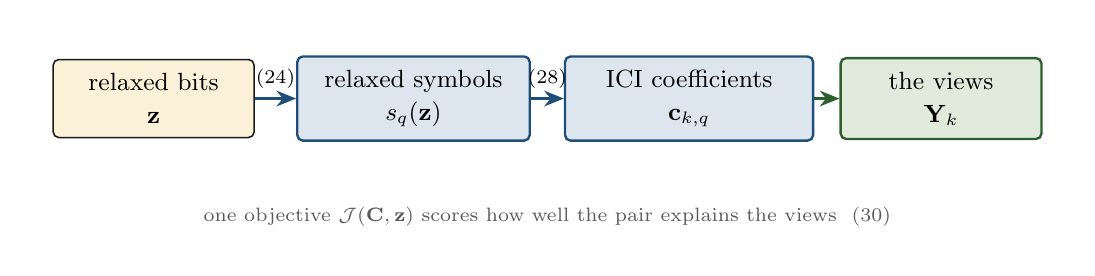
\begin{tikzpicture}[x=1cm,y=1cm]
    \path[use as bounding box] (-6.6,-1.6) rectangle (6.6,1.2);
    \node[card,text width=2.2cm] (bits) at (-5.0,0.3)
      {relaxed bits\\[0.1em]$\mathbf z$};
    \node[bluecard,text width=2.6cm] (sym) at (-1.7,0.3)
      {relaxed symbols\\[0.1em]$s_q(\mathbf z)$};
    \node[bluecard,text width=2.8cm] (coef) at (1.8,0.3)
      {ICI coefficients\\[0.1em]$\mathbf c_{k,q}$};
    \node[goodcard,text width=2.2cm] (views) at (5.0,0.3)
      {the views\\[0.1em]$\mathbf Y_k$};
    \draw[bluearr] (bits) -- (sym) node[midway,above,font=\scriptsize] {(24)};
    \draw[bluearr] (sym) -- (coef) node[midway,above,font=\scriptsize] {(28)};
    \draw[greenarr] (coef) -- (views);
    \node[font=\scriptsize\color{inkgray}] at (0,-1.2)
      {one objective $\mathcal J(\mathbf C,\mathbf z)$ scores how well the
       pair explains the views~~(30)};
  \end{tikzpicture}
\end{frame}

% =====================================================================
% 2. The relaxed QPSK symbol -- (24)
% =====================================================================
\begin{frame}{The relaxed QPSK symbol}
  \centering
  \begin{tikzpicture}[x=1cm,y=1cm]
    \path[use as bounding box] (-6.6,-2.9) rectangle (6.6,2.4);

    \begin{scope}[shift={(-2.5,0.55)},scale=1.0]
      % cube wireframe: the eight edges off the z=-1 face
      \draw[line width=0.4pt,color=inkgray!60]
        (1.42,1.30) -- (-0.58,1.30)
        (1.42,1.30) -- (1.42,-0.70)
        (1.42,-0.70) -- (-0.58,-0.70)
        (-0.58,1.30) -- (-0.58,-0.70);
      \draw[line width=0.4pt,color=inkgray!60]
        (1.42,1.30) -- (0.58,0.70)
        (1.42,-0.70) -- (0.58,-1.30)
        (-0.58,1.30) -- (-1.42,0.70)
        (-0.58,-0.70) -- (-1.42,-1.30);
      % shaded z=-1 face carrying the four QPSK points
      \draw[line width=0.5pt,color=inkgray,fill=inkgray!12]
        (0.58,0.70) -- (0.58,-1.30) -- (-1.42,-1.30) -- (-1.42,0.70) -- cycle;
      \foreach \x/\y in {0.58/0.70,0.58/-1.30,-1.42/0.70,-1.42/-1.30}{
        \fill[accentblue] (\x,\y) circle (2.4pt);
      }
      \node[anchor=south,font=\scriptsize\color{accentblue}] at (0.15,0.92)
        {$\tfrac{1}{\sqrt2}(+1+\mathrm j)$};
      \node[font=\scriptsize] at (-0.42,-1.55) {$\xi_{i_1(k)}$};
      \node[anchor=east,font=\scriptsize] at (-1.52,-0.30) {$\xi_{i_2(k)}$};

      \only<2->{
        \fill[accentred] (-0.10,0.15) circle (2.4pt);
      }
    \end{scope}

    \node[font=\scriptsize,align=center] at (-2.5,-2.30)
      {hard bits: $\xi_{i}=\pm1$, the four QPSK points};

    \only<2->{
      \node[font=\scriptsize\color{accentred},align=center] at (-2.5,-1.62)
        {relaxed bits: inside the face};
    }

    \node[font=\scriptsize] at (0,-2.70)
      {a parity check ties each bit to bits on other carriers; one such bit gives the third axis};

    \only<3->{
      \node[bluecard,text width=6.3cm] at (3.6,0.55)
        {$\displaystyle s_k(\mathbf z)=\frac{1}{\sqrt 2}
          \left[\xi_{i_1(k)}(\mathbf z)+\mathrm j\,\xi_{i_2(k)}(\mathbf z)\right]$
         \\[0.15em]
         \scriptsize equation (24), where $i_1(k)$ and $i_2(k)$ are the two
         coded bits of data carrier $k$ and $\xi_i=\tanh(z_i/2)$ is the
         relaxed bipolar bit of (21)};
      \node[font=\scriptsize,align=center] at (3.6,-1.55)
        {one relaxed bit gives the real part,\\the other the imaginary part};
    }
  \end{tikzpicture}
  \bottomnote{Hard bits give the four QPSK points, and relaxed bits move the
    symbol inside the square those points span.  Pilot carriers keep their
    known symbols.  The square is one face of the cube the coded bits span.}
\end{frame}

% =====================================================================
% 2b. One parity check halves the cube
% =====================================================================
\begin{frame}{One parity check halves the cube}
  \centering
  \begin{tikzpicture}[x=1cm,y=1cm]
    \path[use as bounding box] (-6.6,-2.9) rectangle (6.6,2.4);

    \begin{scope}[shift={(-3.7,-0.15)},scale=1.05]
      % cube edges
      \foreach \ax/\ay/\bx/\by in {
        1.207/1.105/-0.493/1.105, 0.493/0.595/-1.207/0.595,
        1.207/-0.595/-0.493/-0.595, 0.493/-1.105/-1.207/-1.105,
        1.207/1.105/1.207/-0.595, 0.493/0.595/0.493/-1.105,
        -0.493/1.105/-0.493/-0.595, -1.207/0.595/-1.207/-1.105,
        1.207/1.105/0.493/0.595, 1.207/-0.595/0.493/-1.105,
        -0.493/1.105/-1.207/0.595, -0.493/-0.595/-1.207/-1.105}{
        \draw[line width=0.45pt,color=inkgray!60] (\ax,\ay) -- (\bx,\by);
      }
      % face diagonals joining the codeword corners
      \only<2->{
        \foreach \ax/\ay/\bx/\by in {
          1.207/1.105/0.493/-1.105, 1.207/1.105/-1.207/0.595,
          1.207/1.105/-0.493/-0.595, 0.493/-1.105/-1.207/0.595,
          0.493/-1.105/-0.493/-0.595, -1.207/0.595/-0.493/-0.595}{
          \draw[line width=0.8pt,dashed,color=accentgreen] (\ax,\ay) -- (\bx,\by);
        }
      }
      % corners: codewords green, the rest red
      \foreach \cx/\cy/\lb/\lx/\ly in {1.207/1.105/000/1.447/1.345,
                                       0.493/-1.105/011/0.493/-1.445,
                                       -1.207/0.595/101/-1.447/0.835,
                                       -0.493/-0.595/110/-0.813/-0.711}{
        \fill[accentgreen] (\cx,\cy) circle (0.085);
        \only<2->{\node[font=\tiny,color=accentgreen,anchor=center]
          at (\lx,\ly) {\lb};}
      }
      \foreach \cx/\cy in {0.493/0.595, 1.207/-0.595, -0.493/1.105, -1.207/-1.105}{
        \draw[accentred,line width=0.8pt,fill=paper] (\cx,\cy) circle (0.085);
      }
      \node[font=\scriptsize,color=ink,anchor=north] at (0,-1.55)
        {three relaxed bits span the cube $[-1,1]^3$};
    \end{scope}

    \node[card,text width=4.6cm] at (3.4,1.45)
      {$\mathbf P=\begin{pmatrix}1&1&1\end{pmatrix}$,\qquad
       $\mathbf P\mathbf b^{T}=\mathbf 0$\\[0.15em]
       \scriptsize codewords $000$, $011$, $101$, $110$:\\
       four of the eight corners};
    \only<2->{
      \node[goodcard,text width=4.6cm] at (3.4,-0.25)
        {$\mathcal R_{\mathrm{par}}(\mathbf z)=(1-\xi_1\xi_2\xi_3)^2$\\[0.1em]
         \scriptsize $0$ at a green corner, $4$ at a red one};
    }
    \only<3->{
      \begin{scope}[shift={(3.4,-1.85)}]
        \draw[accentred,line width=0.8pt,fill=redbg] (0,0.45) circle (0.16);
        \foreach \xx/\lb in {-1.1/z_1, 0/z_2, 1.1/z_3}{
          \draw[accentblue,line width=0.7pt,fill=blubg] (\xx,-0.35) circle (0.14);
          \draw[line width=0.5pt,color=inkgray] (0,0.30) -- (\xx,-0.20);
          \node[font=\tiny,anchor=north] at (\xx,-0.52) {$\lb$};
        }
        \node[font=\scriptsize,color=inkgray,anchor=south] at (0,0.72)
          {the same check in the Tanner graph};
      \end{scope}
    }
  \end{tikzpicture}
  \bottomnote{Hard bits give the eight cube corners, and one even parity
    check keeps four.  Every cube edge flips one bit and therefore flips
    parity, so kept corners are never neighbours; they sit on face
    diagonals.  Relaxed bits move inside the cube, and the parity penalty
    pulls them toward the kept corners.}
\end{frame}

% =====================================================================
% 3. One coefficient per path -- (25), (26)
% =====================================================================
\begin{frame}{One coefficient per path}
  \centering
  {\small Read $c_{k,q,m}\triangleq\mathbf e_k^T\mathbf F\mathbf S_m
   \mathbf G\mathbf F^H\mathbf e_q$ from right to left.\par}
  \vspace{0.15cm}
  \begin{tikzpicture}[x=1cm,y=1cm]
    \path[use as bounding box] (-6.6,-2.75) rectangle (6.6,1.6)
;
    \node[card,text width=1.75cm] (eq) at (-5.3,0.8)
      {$\mathbf e_q$\\[0.05em]\scriptsize carrier $q$ only};
    \node[card,text width=1.75cm] (ifft) at (-2.65,0.8)
      {$\mathbf F^H$\\[0.05em]\scriptsize to time samples};
    \node[card,text width=1.75cm] (chan) at (0,0.8)
      {$\mathbf G$\\[0.05em]\scriptsize the channel acts};
    \node[card,text width=1.75cm] (win) at (2.65,0.8)
      {$\mathbf S_m$\\[0.05em]\scriptsize keep segment $m$};
    \node[card,text width=1.75cm] (fft) at (5.3,0.8)
      {$\mathbf e_k^T\mathbf F$\\[0.05em]\scriptsize FFT, read bin $k$};
    \draw[bluearr] (eq) -- (ifft);
    \draw[bluearr] (ifft) -- (chan);
    \draw[bluearr] (chan) -- (win);
    \draw[bluearr] (win) -- (fft);

    \only<2->{
      \node[bluecard,text width=5.6cm] at (-3.1,-1.55)
        {$c_{k,q,m}\triangleq\mathbf e_k^T\mathbf F\mathbf S_m
          \mathbf G\mathbf F^H\mathbf e_q$\\[0.1em]
         \scriptsize equation (25): the coupling from transmitted carrier
         $q$ into view $m$ of carrier $k$};
    }
    \only<3->{
      \node[bluecard,text width=5.6cm] at (3.1,-1.55)
        {$\nu_{k,m}\triangleq\mathbf e_k^T\mathbf F\mathbf S_m\mathbf n$
         \\[0.1em]
         \scriptsize equation (26): the same windowed FFT acts on the
         noise};
    }
  \end{tikzpicture}
  \bottomnote{One number per triple: transmitted carrier $q$, received
    carrier $k$, view $m$.  The receiver estimates these coefficients; it
    never evaluates $\mathbf G$.}
\end{frame}

% =====================================================================
% 4. Each view is a linear mix -- (27)
% =====================================================================
\begin{frame}{Each view is a linear mix}
  \centering
  \begin{tikzpicture}[x=1cm,y=1cm]
    \path[use as bounding box] (-6.6,-2.6) rectangle (6.6,2.0);

    \foreach \q/\xc in {q_1/-4.7,q_2/-3.5,q_3/-2.3}{
      \node[qcell,fill=blubg] at (\xc,1.0) {$c_{k,\q,m}$};
      \node[qcell] at (\xc,0.0) {$X_{\q}$};
    }
    \node[font=\scriptsize] at (-3.5,1.62)
      {one coefficient per transmitted carrier};
    \node[font=\scriptsize] at (-3.5,-0.62) {the transmitted symbols};

    \only<2->{
      \node[font=\large] at (-1.3,0.5) {$\Rightarrow$};
      \node[vcell,fill=grnbg] at (0.0,0.5) {$Y_{k,m}$};
      \node[font=\large] at (1.05,0.5) {$+$};
      \node[vcell] at (2.0,0.5) {$\nu_{k,m}$};
      \node[font=\scriptsize,align=center] at (1.0,-0.62)
        {view $m$ of carrier $k$, plus its windowed noise};
    }

    \only<3->{
      \node[bluecard,text width=7.4cm] at (0,-1.85)
        {$\displaystyle Y_{k,m}=\sum_{q\in\Kset}c_{k,q,m}X_q+\nu_{k,m}$
         \\[0.15em]
         \scriptsize equation (27), where the sum covers the active
         transmitted carriers $q$};
    }
  \end{tikzpicture}
  \bottomnote{Each view is a linear combination of the transmitted symbols
    plus its windowed noise.}
\end{frame}

% =====================================================================
% 5. Stack the views, keep the band -- (28)
% =====================================================================
\begin{frame}{Stack the views, keep the band}
  \centering
  \begin{tikzpicture}[x=1cm,y=1cm]
    \path[use as bounding box] (-6.6,-2.85) rectangle (6.6,2.1);

    \foreach \q/\xc in {-3/-3.4,-2/-2.4,-1/-1.4,0/-0.4,1/0.6,2/1.6,3/2.6}{
      \pgfmathtruncatemacro{\inband}{abs(\q)<=1 ? 1 : 0}
      \ifnum\inband=1
        \node[qcell,fill=blubg] at (\xc,1.2) {\ifnum\q=0 $k$\else $k{+}\q$\fi};
      \else
        \node[qcell,fill=paper,draw=inkgray!60,text=inkgray]
          at (\xc,1.2) {$k{+}\q$};
      \fi
    }
    \draw[cpbrace] (-1.95,1.62) -- (1.15,1.62);
    \node[font=\scriptsize] at (-0.4,2.02)
      {$\mathcal B_K(k)$: $\left|q-k\right|\le K_{\mathrm{ICI}}$};
    \node[font=\scriptsize\color{inkgray}] at (-0.4,0.55)
      {carriers outside the band contribute zero};

    \only<2->{
      \foreach \m/\yc in {1/0.0,2/-0.65,3/-1.30,4/-1.95}{
        \node[vcell,minimum width=0.95cm] at (-5.3,\yc) {$Y_{k,\m}$};
      }
      \draw[cpbrace] (-5.95,0.30) -- (-5.95,-2.28);
      \node[font=\scriptsize,anchor=east,align=right] at (-6.15,-1.0)
        {$\mathbf Y_k$\\stack the\\$M$ views};
    }

    \only<3->{
      \node[bluecard,text width=7.2cm] at (1.0,-1.15)
        {$\displaystyle\mathbf Y_k=\sum_{q\in\mathcal B_K(k)}
          \mathbf c_{k,q}\,s_q(\mathbf z)+\bm\nu_k$\\[0.15em]
         \scriptsize equation (28), where
         $\mathbf c_{k,q}=[c_{k,q,1},\ldots,c_{k,q,M}]^T$ and the unknown
         data symbols are replaced by their relaxed values};
      \node[font=\scriptsize,align=center] at (1.0,-2.45)
        {linear in the coefficients; the symbols enter through the relaxed
         bits\\$K_{\mathrm{ICI}}=0$ recovers a per-carrier model};
    }
  \end{tikzpicture}
  \bottomnote{This is the general forward model of (18) made concrete: the
    views of carrier $k$ mix only the carriers of its local ICI
    neighbourhood.}
\end{frame}

% =====================================================================
% 6. The coefficients sum to the channel coefficient -- (29)
% =====================================================================
\begin{frame}{The coefficients sum to the channel coefficient}
  \centering
  {\small When the windows form a partition of unity,
   $\sum_{m}\mathbf S_m=\mathbf I$.\par}
  \vspace{0.1cm}
  \begin{tikzpicture}[x=1cm,y=1cm]
    \path[use as bounding box] (-6.6,-2.9) rectangle (6.6,2.0);

    \begin{scope}[shift={(-4.9,-1.35)}]
      \draw[bluearr] (0,0) -- (0.95,0.05);
      \draw[bluearr] (0.95,0.05) -- (1.80,0.45);
      \draw[bluearr] (1.80,0.45) -- (2.35,1.15);
      \draw[bluearr] (2.35,1.15) -- (2.50,2.00);
      \node[font=\scriptsize\color{accentblue}] at (0.45,-0.35)
        {$c_{k,q,1}$};
      \node[font=\scriptsize\color{accentblue}] at (2.05,-0.05)
        {$c_{k,q,2}$};
      \node[font=\scriptsize\color{accentblue}] at (3.15,1.55)
        {$\cdots\;c_{k,q,M}$};
      \only<2->{
        \draw[redarr,line width=1.3pt] (0,0) -- (2.50,2.00);
        \node[font=\scriptsize\color{accentred},align=center]
          at (0.75,2.15) {their plain sum: $H_{k,q}$};
      }
    \end{scope}

    \only<3->{
      \node[bluecard,text width=6.4cm] at (3.3,0.35)
        {$\displaystyle\mathbf 1^{T}\mathbf c_{k,q}
          =\sum_{m=1}^{M}c_{k,q,m}=H_{k,q}$\\[0.15em]
         \scriptsize equation (29): the $M$ per-view coefficients of a
         carrier pair sum to its channel coefficient};
      \node[font=\scriptsize,align=center] at (3.3,-1.25)
        {the same quantity at two resolutions,\\exactly as the views sum to
         the full-FFT bin in (8)};
    }
  \end{tikzpicture}
  \bottomnote{Component $m$ is one arc of the loop of Fig.~1, and the
    channel coefficient is the average of the whole loop; the coefficients
    collect, carrier by carrier, the arcs the views keep.}
\end{frame}

% =====================================================================
% 7. One objective -- (30)
% =====================================================================
\begin{frame}{One objective}
  \centering
  \begin{tikzpicture}[x=1cm,y=1cm]
    \path[use as bounding box] (-6.6,-2.95) rectangle (6.6,2.1);

    \node[goodcard,text width=4.6cm] (sig) at (-4.0,1.1)
      {signal term\\[0.05em]
       $\displaystyle\lambda_{\mathrm d}\sum_{k\in\Kset}
        \Big\|\mathbf Y_k-\!\!\sum_{q\in\mathcal B_K(k)}\!\!
        \mathbf c_{k,q}s_q(\mathbf z)\Big\|_2^2$};
    \node[font=\scriptsize,align=center] at (-4.0,-0.25)
      {the Gaussian likelihood of the views\\under the forward model (28)};

    \only<2->{
      \node[card,text width=3.0cm] (prior) at (0.1,1.1)
        {coefficient prior\\[0.05em]
         $\gamma_C\norm{\mathbf C}_F^2$};
      \node[font=\scriptsize,align=center] at (0.1,-0.25)
        {the zero-mean Gaussian\\prior on $\mathbf C$};
    }
    \only<3->{
      \node[badcard,text width=3.0cm] (par) at (3.6,1.1)
        {parity penalty\\[0.05em]
         $\lambda_{\mathrm p}\,\mathcal R_{\mathrm{par}}(\mathbf z)$};
      \node[font=\scriptsize,align=center] at (3.9,-0.25)
        {carried over from (23);\\vanishes on codewords};
    }

    \only<4->{
      \node[bluecard,text width=11.6cm] at (0,-1.85)
        {$\mathcal J(\mathbf C,\mathbf z)=
          \text{signal term}+\gamma_C\norm{\mathbf C}_F^2
          +\lambda_{\mathrm p}\,\mathcal R_{\mathrm{par}}(\mathbf z)$
         \\[0.15em]
         \scriptsize equation (30): the general objective (23) with
         $\bm\psi=\mathbf C$; a function of the coefficients and the
         relaxed bits alone};
    }
  \end{tikzpicture}
  \bottomnote{Pilot carriers keep their known symbols in $s_q(\mathbf z)$,
    so the pilots constrain the coefficients through the signal term.  The
    combiner weights are not variables of this problem.}
\end{frame}

% =====================================================================
% 8. JUNA-Iterative
% =====================================================================
\begin{frame}{JUNA-Iterative}
  \centering
  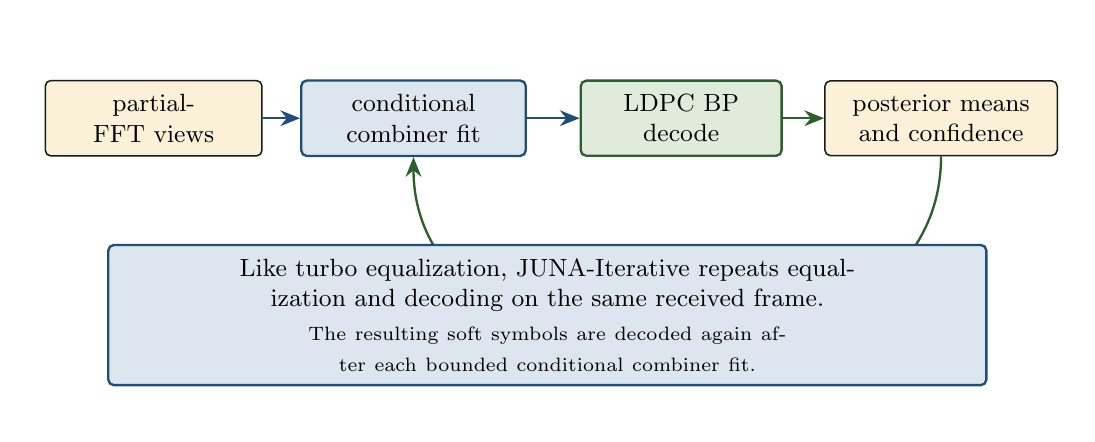
\begin{tikzpicture}[x=1cm,y=1cm]
    \path[use as bounding box] (-6.6,-2.9) rectangle (6.6,2.0);

    \node[card,text width=2.4cm] (views) at (-5.0,0.85)
      {partial-FFT views};
    \node[bluecard,text width=2.5cm] (fit) at (-1.7,0.85)
      {conditional\\combiner fit};
    \node[goodcard,text width=2.2cm] (decode) at (1.7,0.85)
      {LDPC BP\\decode};
    \node[card,text width=2.6cm] (post) at (5.0,0.85)
      {posterior means\\and confidence};
    \draw[bluearr] (views) -- (fit);
    \draw[bluearr] (fit) -- (decode);
    \draw[greenarr] (decode) -- (post);
    \draw[greenarr] (post.south)
      to[out=-90,in=-90,looseness=1.25] (fit.south);

    \node[bluecard,text width=10.8cm] at (0,-1.65)
      {Like turbo equalization, JUNA-Iterative repeats equalization and
       decoding on the same received frame.\\[0.15em]
       \scriptsize The resulting soft symbols are decoded again after each
       bounded conditional combiner fit.};
  \end{tikzpicture}
  \bottomnote{This exchange approximates the joint estimation-and-decoding
    loop motivated by (30).  However, it forms no $\mathbf C$, has no free
    $\mathbf z$, and does not use $\mathcal J$ for step acceptance.}
\end{frame}

% =====================================================================
% 9. JUNA-(C,z)
% =====================================================================
\begin{frame}{JUNA-$C,z$}
  \centering
  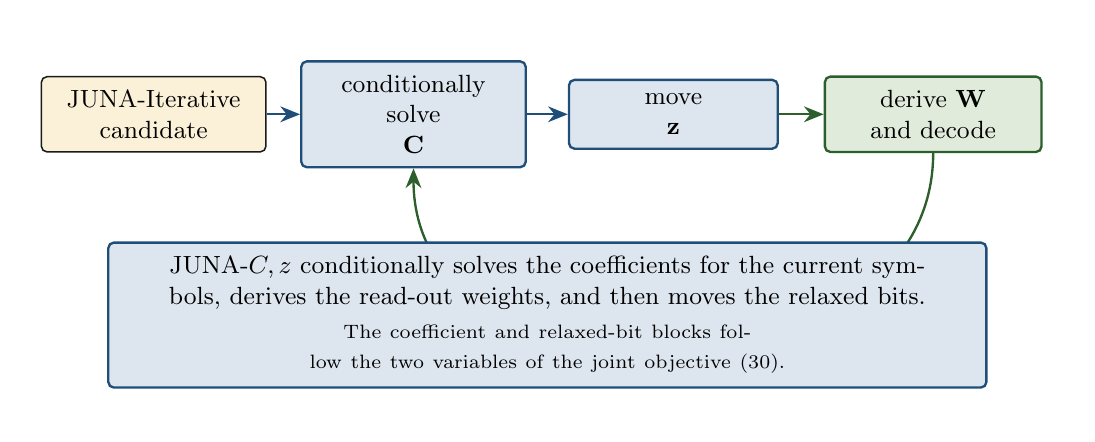
\begin{tikzpicture}[x=1cm,y=1cm]
    \path[use as bounding box] (-6.6,-2.9) rectangle (6.6,2.0);

    \node[card,text width=2.5cm] (iter) at (-5.0,0.9)
      {JUNA-Iterative\\candidate};
    \node[bluecard,text width=2.5cm] (coef) at (-1.7,0.9)
      {conditionally solve\\$\mathbf C$};
    \node[bluecard,text width=2.3cm] (bits) at (1.6,0.9)
      {move\\$\mathbf z$};
    \node[goodcard,text width=2.4cm] (check) at (4.9,0.9)
      {derive $\mathbf W$\\and decode};
    \draw[bluearr] (iter) -- (coef);
    \draw[bluearr] (coef) -- (bits);
    \draw[greenarr] (bits) -- (check);
    \draw[greenarr] (check.south)
      to[out=-90,in=-90,looseness=1.25] (coef.south);

    \node[bluecard,text width=10.8cm] at (0,-1.65)
      {JUNA-$C,z$ conditionally solves the coefficients for the current
       symbols, derives the read-out weights, and then moves the relaxed
       bits.\\[0.15em]
       \scriptsize The coefficient and relaxed-bit blocks follow the two
       variables of the joint objective (30).};
  \end{tikzpicture}
  \bottomnote{This bounded update is motivated by (30).  However, the
    executed rule also contains fixed-reference and decoder terms, so it is
    not identical to $\mathcal J(\mathbf C,\mathbf z)$.}
\end{frame}

% =====================================================================
% 10. JUNA-Direct-(C,z)
% =====================================================================
\begin{frame}{JUNA-Direct-$C,z$}
  \centering
  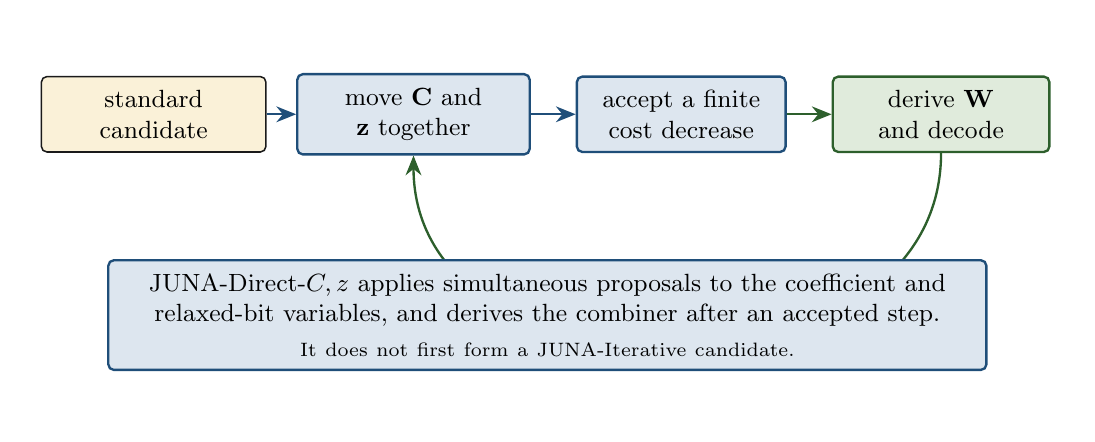
\begin{tikzpicture}[x=1cm,y=1cm]
    \path[use as bounding box] (-6.6,-2.9) rectangle (6.6,2.0);

    \node[card,text width=2.5cm] (start) at (-5.0,0.9)
      {standard\\candidate};
    \node[bluecard,text width=2.6cm] (trial) at (-1.7,0.9)
      {move $\mathbf C$ and\\$\mathbf z$ together};
    \node[bluecard,text width=2.3cm] (accept) at (1.7,0.9)
      {accept a finite\\cost decrease};
    \node[goodcard,text width=2.4cm] (check) at (5.0,0.9)
      {derive $\mathbf W$\\and decode};
    \draw[bluearr] (start) -- (trial);
    \draw[bluearr] (trial) -- (accept);
    \draw[greenarr] (accept) -- (check);
    \draw[greenarr] (check.south)
      to[out=-90,in=-90,looseness=1.25] (trial.south);

    \node[bluecard,text width=10.8cm] at (0,-1.65)
      {JUNA-Direct-$C,z$ applies simultaneous proposals to the coefficient
       and relaxed-bit variables, and derives the combiner after an accepted
       step.\\[0.15em]
       \scriptsize It does not first form a JUNA-Iterative candidate.};
  \end{tikzpicture}
  \bottomnote{JUNA-$C,z$ and JUNA-Direct-$C,z$ use the same variables.
    However, the first conditionally solves the coefficients, whereas the
    second moves both variables together.}
\end{frame}

% =====================================================================
% 11. The posterior-variance alternative -- (68)
% =====================================================================
\begin{frame}{The posterior-variance alternative}
  \centering
  \begin{tikzpicture}[x=1cm,y=1cm]
    \path[use as bounding box] (-6.6,-3.0) rectangle (6.6,2.1);

    \node[card,text width=5.6cm] at (-3.4,1.05)
      {the symbol-error model\\[0.15em]
       $X_q=\mu_q+\varepsilon_q$, with $\mu_q=s_q(\mathbf z)$,\\
       $\E[\varepsilon_q]=0$ and $\E|\varepsilon_q|^2=v_q$};
    \node[font=\scriptsize,align=center] at (-3.4,-0.35)
      {QPSK has unit symbol energy, so $v_q=1-|\mu_q|^2$;\\
       on a pilot or another fixed carrier, $v_q=0$};

    \only<2->{
      \node[bluecard,text width=7.0cm] at (3.15,0.75)
        {$\overline{\mathcal J}_{\mathrm{sig}}
          =\lambda_{\mathrm d}\sum_{k\in\Kset}\Big[
          \big\|\mathbf Y_k-{\textstyle\sum_{q}}
          \mathbf c_{k,q}\mu_q\big\|_2^2
          +{\textstyle\sum_{q}}v_q\norm{\mathbf c_{k,q}}_2^2
          \Big]$\\[0.15em]
         \scriptsize equation (68), with both sums over
         $\mathcal B_K(k)$: the expected signal loss under the
         symbol-error model};
    }
    \only<3->{
      \node[font=\small,align=center] at (0,-1.75)
        {the first term fits the means; the second retains their
         uncertainty};
      \node[font=\scriptsize\color{inkgray},align=center] at (0,-2.45)
        {the larger $v_q$, the more strongly the second term bounds that
         carrier's coefficient energy};
    }
  \end{tikzpicture}
  \bottomnote{It is the posterior-variance alternative and is not used for
    the reported mean-only C,z results; replacing the signal term of (30)
    by (68) gives the complete expected objective.}
\end{frame}

% =====================================================================
% 12. Worked example: the setting
% =====================================================================
\begin{frame}{A worked example}
  \centering
  \begin{tikzpicture}[x=1cm,y=1cm]
    \path[use as bounding box] (-6.6,-2.9) rectangle (6.6,2.0);

    \node[card,text width=5.2cm] at (-3.4,1.05)
      {$N=8$ carriers, $M=4$ views\\[0.1em]
       \scriptsize the channel moves every carrier by a\\
       common offset of $0.20$ bins};
    \node[font=\scriptsize,align=center] at (-3.4,-0.35)
      {with no offset, $\mathbf H=\mathbf I$ exactly:\\
       subcarrier orthogonality};

    \only<2->{
      \node[bluecard,text width=5.6cm] at (3.3,1.05)
        {$\left|H_{4,4}\right|=0.9365$\\[0.1em]
         $\left|H_{4,3}\right|=0.2378\qquad\left|H_{4,5}\right|=0.1618$\\[0.1em]
         \scriptsize the wanted coefficient shrinks and the\\
         neighbouring carriers leak into bin 4};
    }
    \only<3->{
      \node[goodcard,text width=8.6cm] at (0,-1.85)
        {relaxed symbol (24): $\mathbf z=(4,-1)$ gives
         $\xi=(0.9640,\,-0.4621)$\\[0.1em]
         $s=0.6817-0.3268\mathrm j$, so $|s|^2=0.5715$ and
         $v=1-|s|^2=0.4285$ for (68)};
    }
  \end{tikzpicture}
  \bottomnote{Every number in this example is printed by
    \texttt{joint\_tutorial\_worked\_example.py} beside this file, rounded
    to four decimals.}
\end{frame}

% =====================================================================
% 13. Worked example: the split and the view
% =====================================================================
\begin{frame}{The example checks (27) and (29)}
  \centering
  \begin{tikzpicture}[x=1cm,y=1cm]
    \path[use as bounding box] (-6.6,-3.0) rectangle (6.6,2.2);

    \node[card] at (-2.9,0.2)
      {\footnotesize
       \begin{tabular}{@{}lll@{}}
        & $q=4$ (wanted) & $q=5$ (neighbour)\\[0.15em]
        $c_{4,q,1}$ & $0.2485+0.0196\mathrm j$ & $\phantom{-}0.1985+0.1011\mathrm j$\\
        $c_{4,q,2}$ & $0.2303+0.0954\mathrm j$ & $-0.1575+0.1575\mathrm j$\\
        $c_{4,q,3}$ & $0.1895+0.1619\mathrm j$ & $-0.1011-0.1985\mathrm j$\\
        $c_{4,q,4}$ & $0.1302+0.2125\mathrm j$ & $\phantom{-}0.2200-0.0348\mathrm j$\\[0.15em]
        sum & $0.7985+0.4893\mathrm j$ & $\phantom{-}0.1598+0.0253\mathrm j$\\
        $H_{4,q}$ & $0.7985+0.4893\mathrm j$ & $\phantom{-}0.1598+0.0253\mathrm j$
       \end{tabular}};

    \only<2->{
      \node[bluecard,text width=4.9cm] at (4.35,1.15)
        {(29) checks: the sums equal\\$H_{4,q}$ to $2.2\times10^{-16}$
         over all pairs};
      \node[font=\scriptsize,align=center] at (4.35,-0.30)
        {the wanted components add nearly in\\phase; the neighbour
         components point\\in different directions and nearly cancel};
    }
    \only<3->{
      \node[goodcard,text width=11.6cm] at (0,-2.35)
        {(27) checks: view 1 of carrier 4 from the windowed FFT is
         $-0.1396+0.3878\mathrm j$, and from the coefficient mix
         $\sum_q c_{4,q,1}X_q$ it is $-0.1396+0.3878\mathrm j$; they
         differ by $1.1\times10^{-16}$};
    }
  \end{tikzpicture}
  \bottomnote{The coefficients and the windowed FFT are the same
    quantity: one is the model, the other the measurement of it.}
\end{frame}

% =====================================================================
% 14. Worked example: the objective
% =====================================================================
\begin{frame}{The example scores the objective}
  \centering
  \begin{tikzpicture}[x=1cm,y=1cm]
    \path[use as bounding box] (-6.6,-2.9) rectangle (6.6,2.0);

    \node[goodcard,text width=6.0cm] at (-3.2,1.15)
      {signal term at the true pair\\[0.1em]
       with noise $\sigma=0.05$: $\;0.0185$\\[0.1em]
       \scriptsize wrong coefficients or wrong bits\\make this residual grow};

    \only<2->{
      \node[card,text width=5.9cm] at (3.4,1.15)
        {one parity check over three bits,\\
         $\xi$ magnitudes $(0.9640,\,0.4621,\,0.9051)$};
      \node[bluecard,text width=10.8cm] at (0,-1.15)
        {\footnotesize
         \begin{tabular}{@{}lll@{}}
          hard bits, even parity & product $+1$ & penalty $0$\\
          relaxed, correct signs & product $+0.4032$ & penalty $0.3561$\\
          relaxed, one wrong sign & product $-0.4032$ & penalty $1.9691$
         \end{tabular}};
    }
    \only<3->{
      \node[font=\scriptsize,align=center] at (0,-2.30)
        {the penalty orders the three cases: satisfied and confident,
         satisfied but uncertain, violated;\\it vanishes exactly on
         codewords --- in the cube, the cases sit at a green corner,
         inside toward a green corner, and toward a red one};
    }
  \end{tikzpicture}
  \bottomnote{The signal term rewards a pair that reproduces the views,
    and the parity penalty rewards relaxed bits that harden toward a
    codeword.}
\end{frame}

% =====================================================================
% 14b. Worked example: one gradient step in full
% =====================================================================
\begin{frame}{The example takes one gradient step}
  \centering
  \begin{tikzpicture}[x=1cm,y=1cm]
    \path[use as bounding box] (-6.6,-2.9) rectangle (6.6,2.0);

    % t=0: carrier 4 before the step, drawn as the z=xi_2 slice of the cube
    \begin{scope}[shift={(-4.3,0.35)},scale=0.85]
      % cube wireframe
      \draw[line width=0.4pt,color=inkgray!60]
        (1.42,1.30) -- (-0.58,1.30)
        (0.58,0.70) -- (-1.42,0.70)
        (1.42,-0.70) -- (-0.58,-0.70)
        (0.58,-1.30) -- (-1.42,-1.30)
        (1.42,1.30) -- (1.42,-0.70)
        (0.58,0.70) -- (0.58,-1.30)
        (-0.58,1.30) -- (-0.58,-0.70)
        (-1.42,0.70) -- (-1.42,-1.30)
        (1.42,1.30) -- (0.58,0.70)
        (1.42,-0.70) -- (0.58,-1.30)
        (-0.58,1.30) -- (-1.42,0.70)
        (-0.58,-0.70) -- (-1.42,-1.30);
      % target face z=-1 and its target corner
      \draw[line width=0.5pt,color=inkgray]
        (0.58,0.70) -- (0.58,-1.30) -- (-1.42,-1.30) -- (-1.42,0.70) -- cycle;
      \fill[accentgreen] (0.58,0.70) circle (0.075);
      % slice square at z=xi_2, offset (-0.1596,-0.1140)
      \draw[dashed,color=inkgray]
        (0.8404,0.8860) -- (0.8404,-1.1140) -- (-1.1596,-1.1140)
        -- (-1.1596,0.8860) -- cycle;
      % variance ring in the slice plane
      % ball = oblique projection of the per-bit uncertainty ball
      \fill[redbg,opacity=0.75,rotate around={35.5:(0.2203,0.2659)}] (0.2203,0.2659) ellipse ({1.0409} and {0.9250});
      \draw[dashed,color=accentred,rotate around={35.5:(0.2203,0.2659)}] (0.2203,0.2659) ellipse ({1.0409} and {0.9250});
      % slice corners drawn after the ring so they stay visible
      \fill[accentblue] (0.8404,0.8860) circle (0.06);
      \fill[accentblue] (0.8404,-1.1140) circle (0.06);
      \fill[accentblue] (-1.1596,0.8860) circle (0.06);
      \fill[accentblue] (-1.1596,-1.1140) circle (0.06);
      \fill[accentred] (0.2203,0.2659) circle (0.07);
      \only<2->{\draw[greenarr] (0.2203,0.2659) -- (0.58,0.70);}
      \node[font=\scriptsize,align=center] at (0,-1.95)
        {$t=0$: $z_4=(0.8000,0.8000)$\\
         $\xi_4=(0.3799,0.3799)$\\
         $v_4=0.8556$, $\xi_2=-0.3799$};
    \end{scope}

    \node[card,text width=3.55cm,font=\scriptsize] at (0,1.30)
      {carrier 4 sits at\\$s_4=0.2687+0.2687\mathrm j$;\\
       $\mathcal J=3.5608$};
    \only<2->{
      \node[goodcard,text width=3.55cm,font=\scriptsize] at (0,-0.05)
        {the gradient at $z_4$ is\\$(-0.2638,-0.2451)$;\\
         with $\eta=0.8$ the move is\\$(+0.2110,+0.1961)$};
    }
    \only<3->{
      \node[bluecard,text width=3.55cm,font=\scriptsize] at (0,-1.50)
        {the logits grow, the tanh\\hardens, the ring shrinks,\\
         and $\mathcal J$ falls to $2.6663$};
    }

    % t=1: carrier 4 after the step, the slice one step deeper
    \only<3->{
      \begin{scope}[shift={(4.3,0.35)},scale=0.85]
        % cube wireframe
        \draw[line width=0.4pt,color=inkgray!60]
          (1.42,1.30) -- (-0.58,1.30)
          (0.58,0.70) -- (-1.42,0.70)
          (1.42,-0.70) -- (-0.58,-0.70)
          (0.58,-1.30) -- (-1.42,-1.30)
          (1.42,1.30) -- (1.42,-0.70)
          (0.58,0.70) -- (0.58,-1.30)
          (-0.58,1.30) -- (-0.58,-0.70)
          (-1.42,0.70) -- (-1.42,-1.30)
          (1.42,1.30) -- (0.58,0.70)
          (1.42,-0.70) -- (0.58,-1.30)
          (-0.58,1.30) -- (-1.42,0.70)
          (-0.58,-0.70) -- (-1.42,-1.30);
        % target face z=-1 and its target corner
        \draw[line width=0.5pt,color=inkgray]
          (0.58,0.70) -- (0.58,-1.30) -- (-1.42,-1.30) -- (-1.42,0.70) -- cycle;
        \fill[accentgreen] (0.58,0.70) circle (0.075);
        % slice square at z=xi_2, offset (-0.1985,-0.1418)
        \draw[dashed,color=inkgray]
          (0.8015,0.8582) -- (0.8015,-1.1418) -- (-1.1985,-1.1418)
          -- (-1.1985,0.8582) -- cycle;
        % variance ring in the slice plane
        % ball = oblique projection of the per-bit uncertainty ball
        \fill[redbg,opacity=0.75,rotate around={36.2:(0.2679,0.3188)}] (0.2679,0.3188) ellipse ({0.9956} and {0.8866});
        \draw[dashed,color=accentred,rotate around={36.2:(0.2679,0.3188)}] (0.2679,0.3188) ellipse ({0.9956} and {0.8866});
        % slice corners drawn after the ring so they stay visible
        \fill[accentblue] (0.8015,0.8582) circle (0.06);
        \fill[accentblue] (0.8015,-1.1418) circle (0.06);
        \fill[accentblue] (-1.1985,0.8582) circle (0.06);
        \fill[accentblue] (-1.1985,-1.1418) circle (0.06);
        \fill[accentred] (0.2679,0.3188) circle (0.07);
        \node[font=\scriptsize,align=center] at (0,-1.95)
          {$t=1$: $z_4=(1.0110,0.9961)$\\
           $\xi_4=(0.4664,0.4606)$\\
           $v_4=0.7852$, $\xi_2=-0.4727$};
      \end{scope}
    }
  \end{tikzpicture}
  \bottomnote{One plain gradient step on the worked example, printed by the
    same script.  The signal term pulls the symbol toward its corner, the
    parity penalty pushes the $\xi$ magnitudes toward one, and the
    carrier's square rides the check bit: the slice slides toward the
    $\xi_2=-1$ face while the uncertainty ball shrinks around the
    triple.  The ball is a sphere exactly when the three bits are
    equally uncertain --- as at $t=0$ --- and it is axis-aligned
    because the model has no parity correlations.}
\end{frame}

% =====================================================================
% 14b2. Worked example: the same step inside the cube
% =====================================================================
\begin{frame}{The example steps inside the cube}
  \centering
  \begin{tikzpicture}[x=1cm,y=1cm]
    \path[use as bounding box] (-6.6,-2.9) rectangle (6.6,2.4);

    \begin{scope}[shift={(-3.6,-0.15)},scale=1.55]
      \foreach \ax/\ay/\bx/\by in {
        1.207/1.105/-0.493/1.105, 0.493/0.595/-1.207/0.595,
        1.207/-0.595/-0.493/-0.595, 0.493/-1.105/-1.207/-1.105,
        1.207/1.105/1.207/-0.595, 0.493/0.595/0.493/-1.105,
        -0.493/1.105/-0.493/-0.595, -1.207/0.595/-1.207/-1.105,
        1.207/1.105/0.493/0.595, 1.207/-0.595/0.493/-1.105,
        -0.493/1.105/-1.207/0.595, -0.493/-0.595/-1.207/-1.105}{
        \draw[line width=0.4pt,color=inkgray!60] (\ax,\ay) -- (\bx,\by);
      }
      \foreach \cx/\cy in {1.207/1.105, 0.493/-1.105, -1.207/0.595}{
        \fill[accentgreen] (\cx,\cy) circle (0.065);
      }
      \fill[accentgreen] (-0.493,-0.595) circle (0.075);
      \node[font=\scriptsize,color=accentgreen,anchor=west]
        at (-0.42,-0.66) {corner $110$};
      \foreach \cx/\cy in {0.493/0.595, 1.207/-0.595, -0.493/1.105, -1.207/-1.105}{
        \draw[accentred,line width=0.6pt,fill=paper] (\cx,\cy) circle (0.065);
      }
      % trajectory of the triple (xi_2, xi_3, xi_8)
      \only<2->{\draw[greenarr] (-0.187,-0.226) -- (-0.44,-0.53);}
      \fill[accentred] (-0.187,-0.226) circle (0.07);
      \node[font=\tiny,color=accentred,anchor=south west] at (-0.16,-0.20)
        {$t=0$};
      \only<3->{
        \fill[accentred!80] (-0.235,-0.281) circle (0.055);
        \fill[accentred!65] (-0.270,-0.321) circle (0.05);
        \fill[accentred!50] (-0.362,-0.430) circle (0.05);
        \node[font=\tiny,color=accentred!70,anchor=west] at (-0.335,-0.475)
          {$t=8$};
      }
    \end{scope}

    \node[card,text width=4.55cm,font=\scriptsize] at (3.55,1.55)
      {the check over bits $(2,3,8)$;\\its codeword corner is $110$\\[0.1em]
       $\boldsymbol\xi=(-0.3799,\,-0.3799,\,0.3799)$\\
       penalty $0.8933$,\quad $\mathcal J=3.5608$};
    \only<2->{
      \node[goodcard,text width=4.55cm,font=\scriptsize] at (3.55,0.05)
        {the gradient on the triple is\\$(0.2839,\,0.2765,\,-0.2638)$;\\
         with $\eta=0.8$ the move is\\$(-0.2271,\,-0.2212,\,+0.2110)$\\
         --- toward corner $110$};
    }
    \only<3->{
      \node[bluecard,text width=4.55cm,font=\scriptsize] at (3.55,-1.55)
        {after eight steps\\$\boldsymbol\xi=(-0.7243,\,-0.7191,\,0.7098)$\\
         penalty $0.3973$,\quad $\mathcal J=0.8446$\\[0.1em]
         the penalty falls at every step};
    }
  \end{tikzpicture}
  \bottomnote{The same gradient step drawn in bit space: the signal term
    pulls each symbol toward its QPSK corner, and the parity penalty steers
    the triple toward its codeword corner.  The trajectory stays inside the
    cube because the tanh bounds every $\xi$.}
\end{frame}

% =====================================================================
% 14c. Worked example: the variance evolution
% =====================================================================
\begin{frame}{The example shrinks the variance}
  \centering
  \begin{tikzpicture}[x=1cm,y=1cm]
    \path[use as bounding box] (-6.6,-2.9) rectangle (6.6,2.0);

    \foreach \on/\xo/\tl/\sxa/\sya/\sxb/\syb/\px/\py/\ea/\eb/\ang/\vv/\jj in {
        1/-5.0/$t=0$/-1.1596/-1.1140/0.8404/0.8860/0.2203/0.2659/1.0409/0.9250/35.5/0.8556/3.5608,
        2/-2.5/$t=1$/-1.1985/-1.1418/0.8015/0.8582/0.2679/0.3188/0.9956/0.8866/36.2/0.7852/2.6663,
        3/0.0/$t=2$/-1.2267/-1.1619/0.7733/0.8381/0.3032/0.3586/0.9547/0.8519/37.0/0.7241/2.0942,
        4/2.5/$t=4$/-1.2641/-1.1886/0.7359/0.8114/0.3518/0.4144/0.8874/0.7942/38.3/0.6286/1.4296,
        5/5.0/$t=8$/-1.3042/-1.2173/0.6958/0.7827/0.4056/0.4775/0.7942/0.7137/40.2/0.5067/0.8446}{
      \only<\on->{
        \begin{scope}[shift={(\xo,0.55)}]
          \begin{scope}[scale=0.42]
            \draw[line width=0.5pt,color=inkgray]
              (-1.42,-1.30) rectangle (0.58,0.70);
            \fill[accentgreen] (0.58,0.70) circle (0.18);
            \draw[dashed,color=inkgray] (\sxa,\sya) rectangle (\sxb,\syb);
            \fill[redbg,opacity=0.75,rotate around={\ang:(\px,\py)}] (\px,\py) ellipse ({\ea} and {\eb});
            \draw[dashed,color=accentred,rotate around={\ang:(\px,\py)}] (\px,\py) ellipse ({\ea} and {\eb});
            \fill[accentblue] (\sxa,\sya) circle (0.12);
            \fill[accentblue] (\sxa,\syb) circle (0.12);
            \fill[accentblue] (\sxb,\sya) circle (0.12);
            \fill[accentblue] (\sxb,\syb) circle (0.12);
            \fill[accentred] (\px,\py) circle (0.14);
          \end{scope}
          \node[font=\scriptsize\bfseries,anchor=south] at (0,0.95) {\tl};
          \node[font=\scriptsize,color=accentred,anchor=north] at (0,-1.02)
            {$v_4=\vv$};
          \node[font=\scriptsize,color=accentblue,anchor=north] at (0,-1.42)
            {$\mathcal J=\jj$};
        \end{scope}
      }
    }
    \only<2->{\draw[bluearr] (-4.20,0.55) -- (-3.35,0.55);}
    \only<3->{\draw[bluearr] (-1.70,0.55) -- (-0.85,0.55);}
    \only<4->{\draw[bluearr] (0.80,0.55) -- (1.65,0.55);}
    \only<5->{\draw[bluearr] (3.30,0.55) -- (4.15,0.55);}

    \only<6->{
      \node[bluecard,text width=7.6cm] at (-1.8,-2.35)
        {every one of the eight steps lowers $\mathcal J$, $v_4$, and
         the mean $v$, which falls from $0.8556$ to $0.4816$};
      \node[font=\scriptsize,align=center] at (4.35,-2.35)
        {descent hardens the relaxed bits:\\
         $|\mu_q|$ grows, so $v_q=1-|\mu_q|^2$ falls};
    }
  \end{tikzpicture}
  \bottomnote{Gradient steps on the worked example, printed by the same
    script: the coefficients are held at their true values and plain
    gradient steps with a fixed step size move only $\mathbf z$; the
    receiver instead solves $\mathbf C$ conditionally and moves
    $\mathbf z$ with Adam.  The signal likelihood rises as the objective
    falls.}
\end{frame}

% =====================================================================
% 15. Takeaway
% =====================================================================
\begin{frame}[plain]
  \centering
  \vspace{0.7cm}
  {\bfseries\LARGE The joint demodulation and decoding problem\par}
  \vspace{0.5cm}
  {\large relaxed bits form the symbols~(24); the ICI coefficients carry
   them into the views~(25)--(28)\par}
  \vspace{0.30cm}
  {\large the per-view coefficients sum to the channel coefficient~(29)\par}
  \vspace{0.30cm}
  {\large one objective scores the pair $(\mathbf C,\mathbf z)$~(30)\par}
  \vspace{0.30cm}
  {\large JUNA-Iterative exchanges a conditional combiner fit and decoding;
   JUNA-$C,z$ and JUNA-Direct-$C,z$ move the joint variables\par}
  \vspace{0.30cm}
  {\large the posterior-variance alternative is equation~(68)\par}
  \vspace{0.45cm}
  {\itshape the pilots constrain the coefficients; the parity checks
   constrain the bits; both act in the same objective\par}
\end{frame}

\end{document}
